% This text is proprietary.
% It's a part of presentation made by myself.
% It may not used commercial.
% The noncommercial use such as private and study is free
% Sep. 2010
% Author: Sascha Frank 
% University Freiburg 
% www.informatik.uni-freiburg.de/~frank/
%
% 

\documentclass[handout]{beamer}
\setbeamertemplate{navigation symbols}{}


\usetheme{Warsaw}
\usepackage{ngerman}
\beamersetuncovermixins{\opaqueness<1>{25}}{\opaqueness<2->{15}}
\begin{document}
\title{LES RESEAUX DOMESTIQUES ET LA DOMOTIQUE}  
\author{LAVIER Antoine et NTUMBA wa NTUMBA Patient}
\date{\today} 

\begin{frame}
\titlepage
\end{frame} 

\begin{frame}
\frametitle{Contenu}
\tableofcontents
\end{frame} 


\section{Introduction} 
\begin{frame}\frametitle{Introduction} 
\begin{figure}
		\centering
		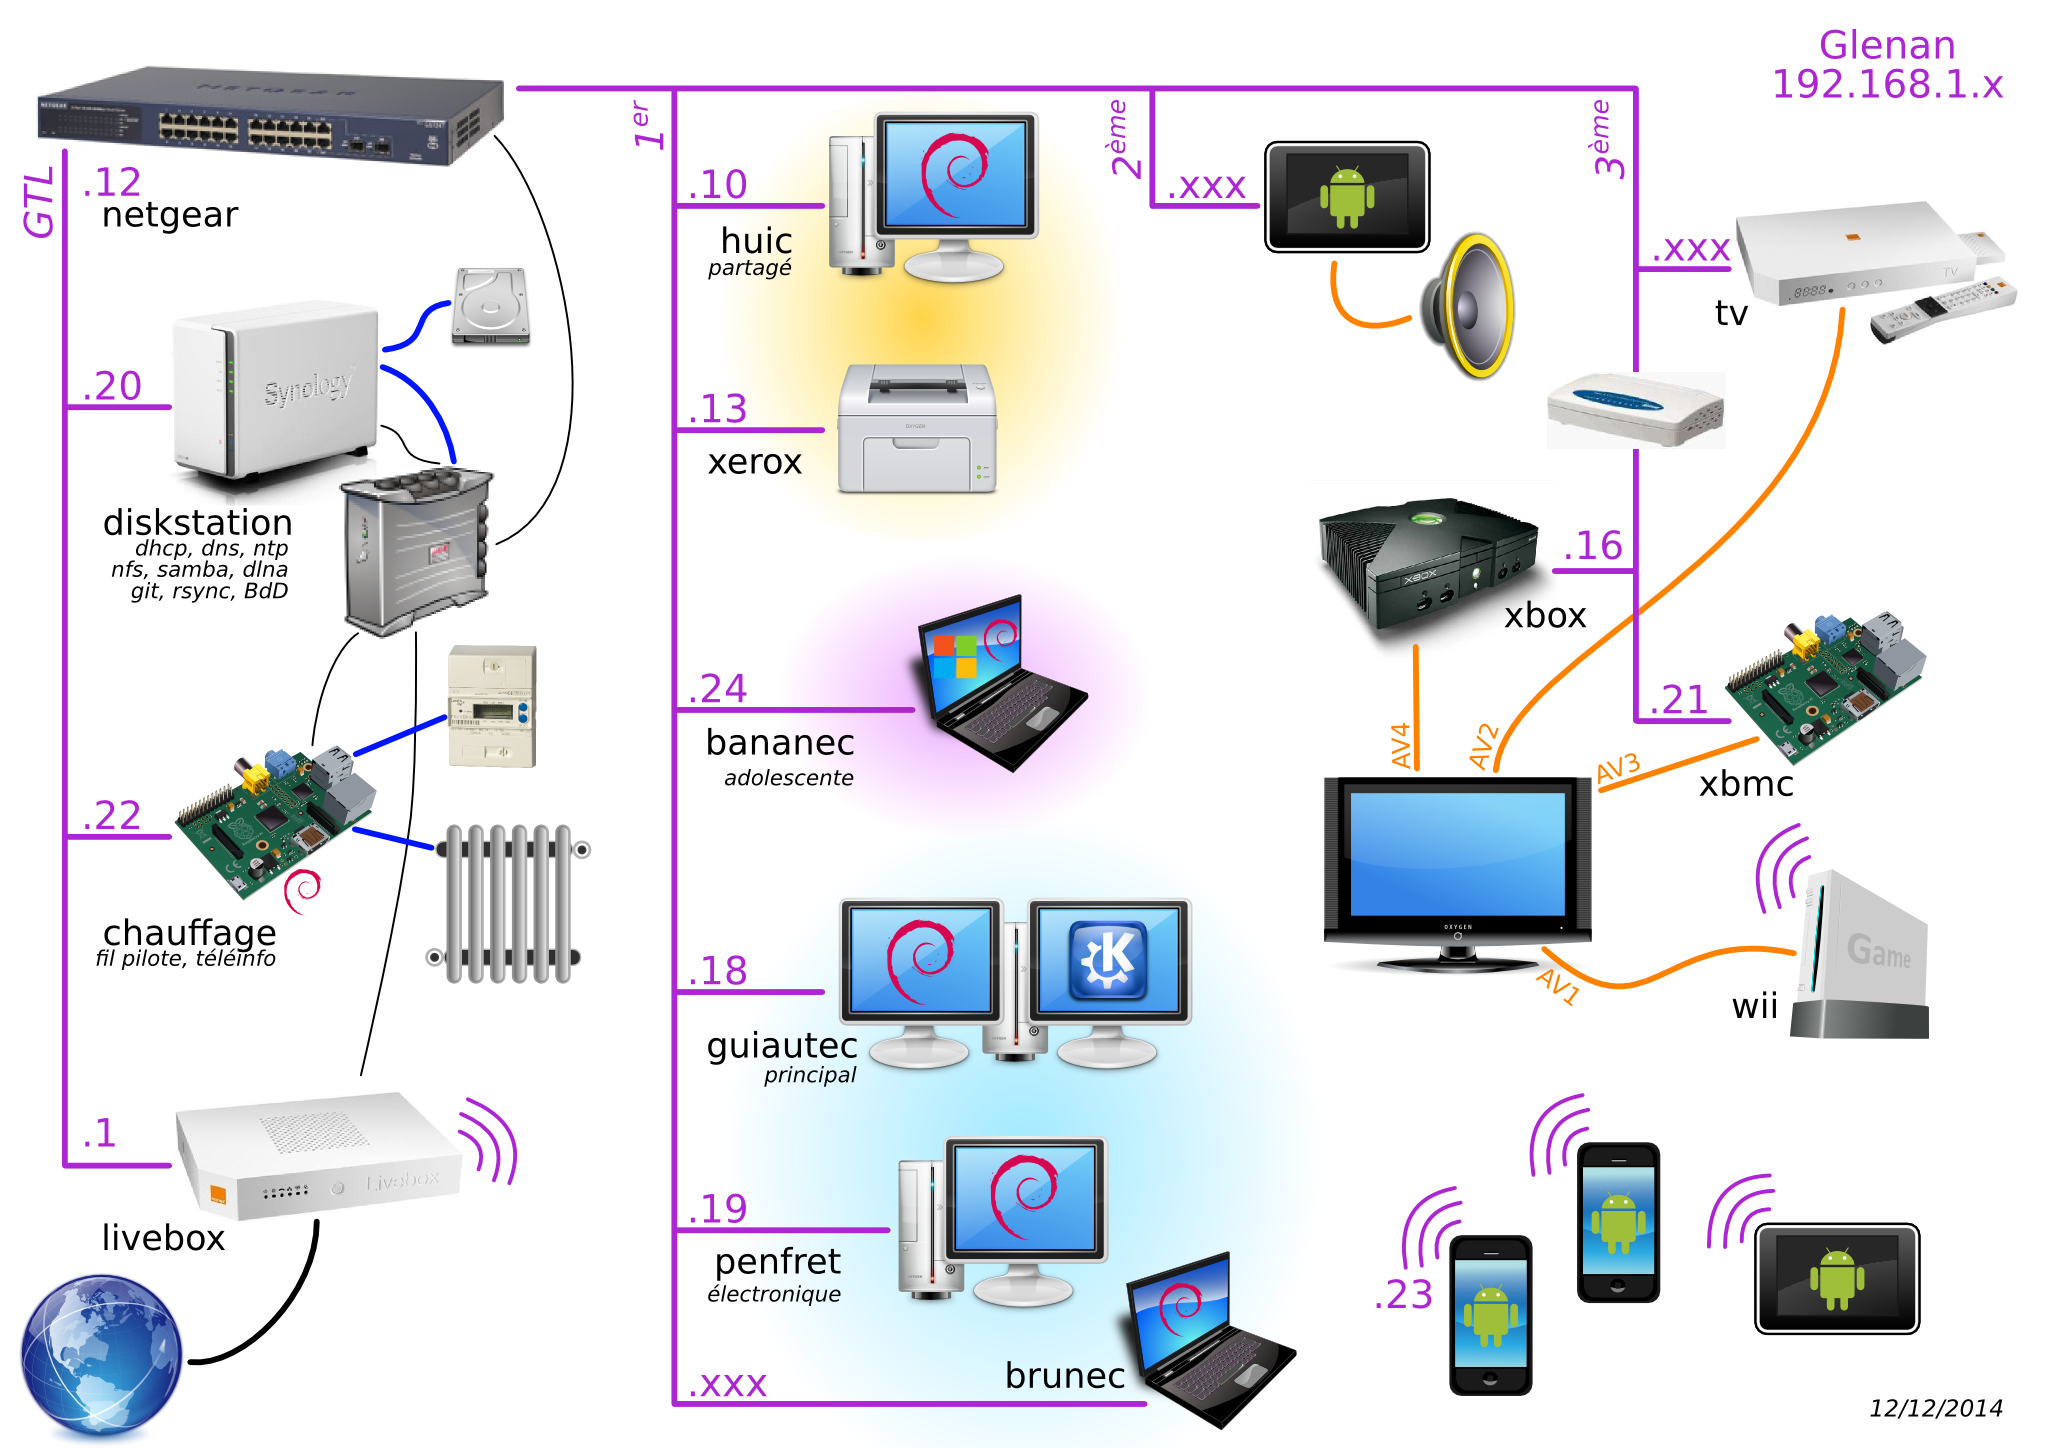
\includegraphics[width=1\textwidth,natwidth=100,natheight=100]{image/LAN6.png}
\end{figure}
\end{frame}
\end{document}
